\chapter{Revisão de conceitos e de bibliografia} \label{sec:revis_biblio}

Neste capítulo descreve-se, primeiramente, o problema de não aderência ao sequenciamento programado e como ele se encaixa no contexto de distribuição de última milha.
Em seguida, serão definidas variáveis de ``circuicidade'', densidade e conectividade no contexto de zonas urbanas, assim como os principais conceitos de regressões lineares.
Tais variáveis e conceitos são apresentados a partir de trabalhos anteriores, que serão mencionados logo em seguida, e, ao longo do presente trabalho, serão utilizados como base para a construção e validação das análises e dos resultados.

Os trabalhos anteriores, que serão mencionados, discorrem acerca da relação entre a rede viária e a eficiência de entregas de última milha, assim como a análise espacial destas malhas por meio de metodologia baseada em grafos. 
Também são descritos alguns dos fundamentos de autocorrelação espacial, que permitirão estabelecer análises de geoestatísticas no decorrer do trabalho. 
Por fim, são apresentadas as considerações finais com respeito à literatura. 

%%%%%%%%%%%%%%%%%%%%%%%%%%%%%%%%%%%%%%%%%%%%%%%%%%%%%%%
\section{Distribuição de última milha em regiões urbanas} \label{sec:definicaoProblema} 

Distribuição de última milha (do inglês \textit{last mile distribution}) refere-se ao último segmento de entrega de mercadorias, ou seja, é a última etapa de uma viagem que vai desde a origem de uma mercadoria até o destino final da entrega.
A distribuição de entregas de última milha em áreas urbanas configura parte importante da engenharia de transportes e também do gerenciamento de cadeias de suprimentos, uma vez que são diversos os estabelecimentos que se beneficiam ou dependem desse tipo de entrega, como supermercados, bares, restaurantes, postos de gasolina, hospitais, entre outros.
Além disso, entregas de última milha em áreas urbanas geralmente são caracterizadas por pequenas distâncias percorridas, elevada quantidade de mercadorias e elevada frequência de entregas, sobretudo em centros urbanos de elevada densidade demográfica.

Empresas que realizam entregas de última milha normalmente enfrentam o problema de roteirização de veículos, que é derivado do termo inglês \textit{Vehicle Routing Problem} (VRP), o qual foi apresentado pela primeira vez por \citeonline{dantzig1959truck}.
De acordo com \citeonline{EKSIOGLU20091472}, a forma clássica do VRP pode ser definida do seguinte modo: 

\singlespacing
\begin{tcolorbox}
\begin{itemize}
    \item Dado um grafo $G=(V,A)$ em que $V$ é um conjunto de $n$ nós em que $V=\{0,1,...,n\}$ e $A$ é o conjunto de arcos;
    \item Os nós $j=1,..., n$ do conjunto $V$ correspondem aos clientes e o nó $j=0$ corresponde ao depósito de origem;
    \item Um custo não negativo é associado a cada arco presente em $A$, sendo que este custo pode representar o tempo ou distância do percurso entre os dois nós que estão conectados pelo arco em questão;
    \item O VRP consiste em encontrar um conjunto de $k$ circuitos (rotas), cada um representando uma rota de mínimo custo, que é definida como a soma de modo que;
    \begin{itemize}
        \item Cada circuito contém o nó $j=0$, ou seja, o depósito;
        \item Cada nó $j$, em que $j \in V\setminus\{0\}$ é visitado por exatamente um único circuito e
        \item a soma das demandas de cada nó em uma rota não supera a capacidade $C$ do veículo.
    \end{itemize}
\end{itemize}
\end{tcolorbox}
\onehalfspacing

A título de observação, quando há somente um único veículo e o objetivo é minimizar a distância total percorrida, o VRP se reduz ao Problema do Caixeiro Viajante, do inglês \textit{Travelling Salesman Problem} (TSP) que por sua vez, de acordo com \citeonline{cookTSP}, não possui uma origem muito bem definida pela literatura. 

Desde a concepção do VRP em \citeyear{dantzig1959truck}, diversas soluções já foram formuladas na literatura, sendo a maior parte delas, segundo \citeonline{BRAEKERS2016300}, baseada em algoritmos de metaheurística, visto que o VRP é um problema de complexidade NP-difícil (\citeauthoronline{garey1976some}, \citeyear{garey1976some}), ou \textit{NP-hard}.
Conforme discutido por \citeonline{arora2009computational}, problemas do tipo \textit{NP-hard} não possuem algoritmo eficiente que resolva, em tempo polinomial, o seu caso mais difícil possível. 
Em outras palavras, conforme o número de pontos a serem visitados aumenta, o esforço computacional empregado para se resolver o VRP cresce exponencialmente, tornando teoricamente impossível a solução ótima quando o número de pontos tende ao infinito. 
% The fact that a problem is NP-hard means that we believe there is no efficient algorithm that solves it in the worst case. It does not, however, mean that every single instance of the problem is hard

Exemplos de metaheurísticas utilizadas para solucionar o VRP podem ser amplamente encontrados na literatura, como é o caso das soluções apresentadas por \citeonline{chiang1997reactive} e \citeonline{homberger1999two}, por exemplo.
Em geral, estes algorítimos baseados em metaheurísticas podem reduzir significativamente o tempo de processamento ao se resolver o VRP (\citeauthoronline{Golden1998}, \citeyear{Golden1998}).
Essa redução de tempo é o que permite que grandes empresas possam otimizar os roteiros de entregas e aumentar o desempenho de suas operações, muitas das vezes atingindo impactos notáveis, como é o caso das aplicações ORION (\citeauthoronline{holland2017ups}, \citeyear{holland2017ups}) e SHORTREC (\citeauthoronline{kant2008coca}, \citeyear{kant2008coca}) desenvolvidas pelas empresas \textit{UPS} e \textit{Coca-Cola}, respectivamente, e que permitiram atingir uma economia anual de \$300 milhões e \$45 milhões de dólares, respectivamente.

Contudo, muitas vezes os resultados das roteirizações não podem ser executados exatamente como programado durante a operação de entregas.
Essa diferença pode ser representada por distâncias adicionais percorridas, tempo adicional de entregas ou até mesmo sequência de visitas em ordem diferente da que foi programada.
A esse fenômeno dá-se o nome de ``não aderência ao sequenciamento programado'', que será o principal objeto de estudo deste trabalho.

%%%%%%%%%%%%%%%%%%%%%%%%%%%%%%%%%%%%%%%%%%%%%%%%%%%%%%%
\section{O fator de circuito} \label{sec:fatorCircuito}
Fator de circuito, ou \textit{circuity factor} em inglês, pode ser definido como a razão entre a menor distância a ser percorrida por um veículo ao ir de um ponto a outro da cidade e a distância euclidiana, isto é, em linha reta entre estes mesmos dois pontos. 
A Equação \ref{eq:fator_circuito} descreve o cálculo do fator de circuito entre dois pontos $p$ e $q$ genéricos.
%
\begin{equation} \label{eq:fator_circuito}
    C_{f_{p, q}} = \frac{(Dist\hat{a}ncia\;Real)_{p, q}}{(Dist\hat{a}ncia\;Euclidiana)_{p, q}}
\end{equation}

Valores de $C_{f}$ podem variar de $1$ até, teoricamente, infinito visto que, para um plano, a distância real percorrida jamais poderá ser menor do que a distância em linha reta entre dois pontos.
Porém é importante destacar que conforme a distância euclidiana aumenta, a distância real percorrida tende a se aproximar cada vez mais da distância em linha reta entre estes dois pontos, conforme ilustrado pela Equação (\ref{eq:limite}).
%
\begin{equation} \label{eq:limite}
    \lim_{Dist\hat{a}ncia\;Euclidiana \rightarrow \infty} \frac{Dist\hat{a}ncia\;Real}{Dist\hat{a}ncia\;Euclidiana} = 1
\end{equation}

De fato, a Figura \ref{fig:FC_julia_artigo} ilustra essa relação assintótica do fator de circuito, onde o eixo das abscissas indica a distância euclidiana e o eixo das ordenadas representa o fator de circuito.
O fator de circuito pode representar a eficiência de locomoção de veículos em zonas urbanas, visto que em geral malhas com fatores de circuito menores representam maior agilidade ao se movimentar por diferentes trechos, ou seja, exigindo menos esforço para se realizar um determinado percurso.

\begin{figure}[H]
    \centering
    \caption{Exemplo de fator de circuito calculado para a cidade de Nova Iorque.}
    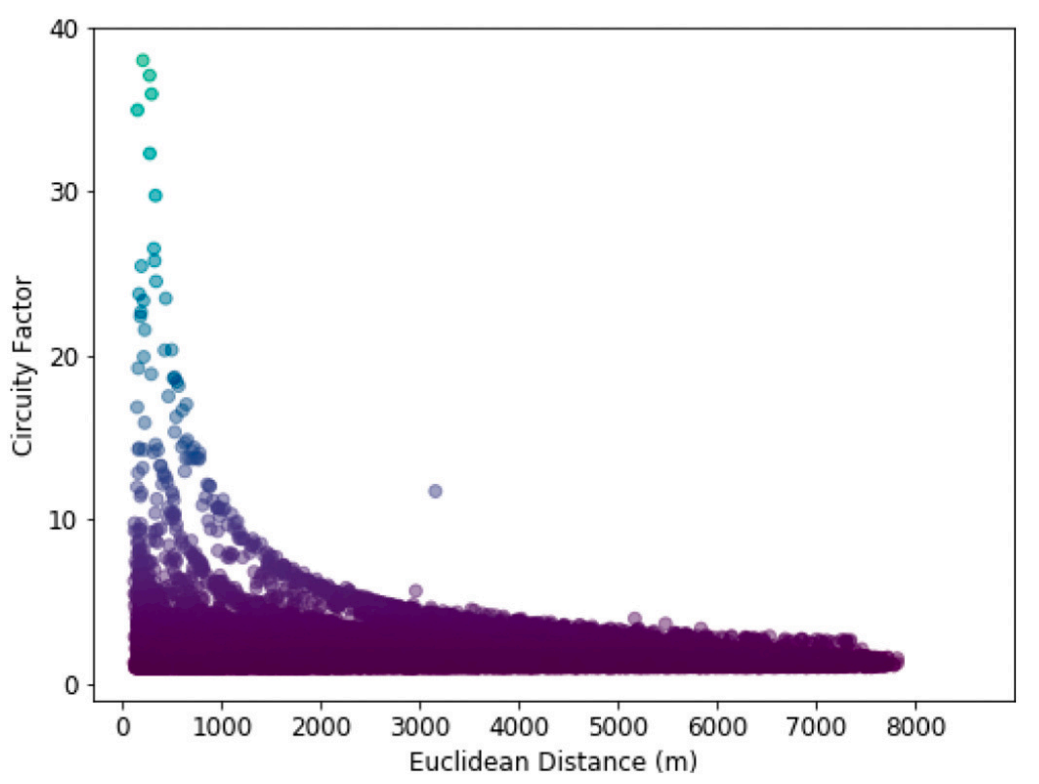
\includegraphics[width=.4\linewidth]{images/2_revisao/julia_fc.png}
    \caption*{\ Fonte: \citeonline{AMARAL2020102916}}
    \label{fig:FC_julia_artigo}
\end{figure}

%%%%%%%%%%%%%%%%%%%%%%%%%%%%%%%%%%%%%%%%%%%%%%%%%%%%%%%
\section{Densidade e conectividade de malhas urbanas} \label{sec:DensConectBiblio}

As medidas descritas nesta seção buscam caracterizar valores com respeito à densidade e conectividade das malhas urbanas, e serão utilizadas com este mesmo propósito ao longo do trabalho.
Densidade se refere à concentração de determinados elementos (e.g. vias e intersecção) na malha urbana, enquanto conectividade refere-se ao quão interligados estão estes elementos da malha viária.
As definições utilizadas podem apresentar variações pela literatura, porém, em geral optou-se por adotar, neste trabalho, a forma padrão de cada um dos indicadores.
Inicialmente apresenta-se o índice de conectividade $C_{index}$ (\citeauthoronline{Marshall_metrics}, \citeyear{Marshall_metrics}), descrito na Equação \ref{eq:conectivity_index} e que representa a razão entre o número de segmentos de vias e o número total de intersecções em uma malha viária.
%
\begin{equation} \label{eq:conectivity_index}
    C_{index} = \frac{n^{\circ}\;de\;Segmentos\;de\;via}{n^{\circ}\;de\;Intersecc\tilde{o}es}
\end{equation}

Também apresenta-se a densidade de intersecções $D_{Intsec}$ (\citeauthoronline{Marshall_metrics}, \citeyear{Marshall_metrics}), que é definida como sendo a divisão entre o número total de intersecções e a área total da malha urbana estudada, conforme descrito na Equação \ref{eq:intersec_density}.
%
\begin{equation} \label{eq:intersec_density}
    D_{Intsec} = \frac{n^{\circ}\;de\;Intersecc\tilde{o}es}{Area}
\end{equation}

Assim como feito para a densidade de intersecções, podemos definir a densidade de vias ($D_{vias}$) como sendo o comprimento total de vias dividido pela área total da malha, conforme a Equação \ref{eq:streets_density}.
%
\begin{equation} \label{eq:streets_density}
    D_{Vias} = \frac{Comprimento \; total \; de \; vias}{Area}
\end{equation}

Por fim, define-se a proporção de vias de mão única ($OW_{ratio}$), a qual reflete o percentual de vias que possuem um único sentido de trafego em relação ao total de vias da malha urbana.  
%
\begin{equation} \label{eq:ow_ratio}
    OW_{ratio}(\%) = 100 \cdot \frac{n^{\circ}\;de\;vias\;de\;m\tilde{a}o\;unica}{n^{\circ}\;de\;vias}
\end{equation}

Quando combinadas, as variáveis apresentadas nesta seção podem fornecer uma descrição preliminar da geometria da malha viária. 
Contudo, posteriormente outras variáveis serão definidas, de modo a ser obter uma descrição mais completa.
Conforme apontado por \citeonline{Marshall_metrics}, algumas dessas medidas de conectividade ($C_{index}$, $D_{Intsec}$ e $D_{Vias}$) podem apresentar inconsistências ao se representar a conectividade de malhas viárias, isso por conta de elas serem funções não lineares da área e geometria das vias. 

%%%%%%%%%%%%%%%%%%%%%%%%%%%%%%%%%%%%%%%%%%%%%%%%%%%%%%%
\section{Regressões lineares} \label{RegressoesLineares}

Tratando-se de regressões lineares simples, \citeonline{Azevedo2016} descreve que para identificar a possível dependência entre duas variáveis $X$ e $Y$, pode-se escrever uma combinação linear tal como apresentada na Equação \ref{eq:reg_linear1}, onde  $Y$ é a variável dependente, $X$ é a variável preditora, $\beta_{0}$ e $\beta_{1}$ são parâmetros de ajuste a serem definidos e $\epsilon_{i}$ é o erro associado ao ajuste da regressão aos dados observados. 
Quanto maior a acurácia da regressão, menor é o valor de $\epsilon_{i}$.
%
\begin{equation} \label{eq:reg_linear1}
    Y = \beta_{0}+\beta_{1}\cdot X+\epsilon_{i}
\end{equation}

\citeonline{Azevedo2016} indica que a chave para a construção de uma regressão linear simples é a definição de $\beta_{0}$ e $\beta_{1}$, os quais podem ser calculados através do métodos de mínimos quadrados (\citeauthoronline{BJORCK1990465}, \citeyear{BJORCK1990465}).
O método dos mínimos quadrados consiste em definir os parâmetros $\beta_{0}$ e $\beta_{1}$ de modo a minimizar o valor absoluto de $\epsilon_{i}$. 
Além disso, ele também define variáveis relacionadas à qualidade da regressão. 
Primeiramente, é estabelecida a soma dos quadrados total (SQT), definida na Equação \ref{eq:reg_linear2}, onde $n$ é a quantidade de observações utilizadas para a construção da regressão. 
Assim, a SQT mensura a variação total de $Y_{i}$.
%
\begin{equation} \label{eq:reg_linear2}
    SQT = \sum_{i=1}^{n} \quad (Y_{i} - \overline{Y})^2 = \sum_{i=1}^{n} \quad Y_{i}^2 - n\overline{Y}^2
\end{equation}

Alternativamente, a variação total de $Y_{i}$ também pode ser representada pela soma dos quadrados dos erros (SQE), conforme apresentado na Equação \ref{eq:reg_linear3}.
%
\begin{equation} \label{eq:reg_linear3}
    SQE = \sum_{i=1}^{n} \quad (Y_{i} - \hat{Y}_{i})^2
\end{equation}

Por fim, ambas as somas SQT e SQE são associadas conforme a Equação \ref{eq:reg_linear4}, tornando possível construir um indicador denominado coeficiente de determinação ($r^2$). 
\citeonline{Azevedo2016} explica que o termo $r^2$ pode ser interpretado como ``a proporção da variação total de Y que é explicada por X, segundo o modelo de regressão considerado.''.
O valor do $r^2$ pode variar de 0 a 1, sendo $r^{2}=0$ um nível total de independência entre $X$ e $Y$, e $r^{2}=1$ um nível total de dependência entre $X$ e $Y$.
%
\begin{equation} \label{eq:reg_linear4}
    r^2 = \frac{SQT-SQE}{SQT}
\end{equation}

Adicionalmente, \citeonline{Chein2019} define regressão linear múltipla, que permite determinar, simultaneamente, a relação que múltiplos preditores (X) têm com a variável dependente (Y). 
Assim, o modelo de regressão linear múltipla é definido como na Equação \ref{eq:reg_linear5}, onde $X_{1}$, $X_{2}$, ..., $X_{k}$ são as $k$ variáveis preditoras do modelo.
%
\begin{equation} \label{eq:reg_linear5}
    Y = \beta_{0}+ \beta_{1} \cdot X_{1} + \beta_{2} \cdot X_{2} + ... + \beta_{k} \cdot X_{k} + \epsilon_{i}
\end{equation}

Assim como feito para as regressões simples, é definido o coeficiente de determinação das regressões múltiplas.
Para tanto, são utilizados os $r^2$ das regressões lineares simples estabelecidas entre os diferentes pares de variáveis Y, $X_{1}$, $X_{2}$, ... e $X_{k}$
A Equação \ref{eq:reg_linear6} apresenta a definição do coeficiente de determinação múltiplo, onde $r_{X_{i}X_{j}}$ é o coeficiente de determinação da regressão linear simples entre $X_{i}$ e $X_{j}$. 
%
\begin{equation} \label{eq:reg_linear6}
    \begin{bmatrix}
    r_{X_{1},X_{2},...,X_{k},Y}^2 
    \end{bmatrix} = 
    \begin{bmatrix}
    r_{X_{1}Y} & r_{X_{2}Y} & ... & r_{X_{k}Y}
    \end{bmatrix} \cdot
    \begin{bmatrix}
    r_{X_{1}X_{1}} & r_{X_{1}X_{2}} & ... & r_{X_{1}X_{k}} \\
    r_{X_{2}X_{1}} & r_{X_{2}X_{2}} & ... & r_{X_{2}X_{k}} \\
    ... & ... & ... & ... \\
    r_{X_{k}X_{1}} & r_{X_{k}X_{2}} & ... & r_{X_{k}X_{k}} \\
    \end{bmatrix}^{-1} \cdot
    \begin{bmatrix}
    r_{X_{1}Y} \\ r_{X_{2}Y} \\ ... \\ r_{X_{k}Y}
    \end{bmatrix}
\end{equation}

Contudo, o coeficiente de determinação da regressão múltipla desconsidera o efeito do número de variáveis preditoras utilizadas na regressão, resultando em valores cada vez maiores de $r^{2}$ conforme se aumenta o número de variáveis, o que pode causar uma falsa afirmação de que as regressões múltiplas necessariamente possuem maior acurácia quando comparado às regressões lineares (\citeauthoronline{Chein2019}, \citeyear{Chein2019}).
Sendo assim, define-se o indicador $r^2_{ajustado}$, o qual considera o número de variáveis preditoras utilizadas no modelo, conforme indicado na Equação \ref{eq:reg_linear7}, onde $n$ é a quantidade de observações utilizadas para construir a regressão e $k$ é o número de variáveis preditoras utilizadas.
%
\begin{equation} \label{eq:reg_linear7}
    r^2_{ajustado} = 1 - (1 - r^2) \cdot \frac{n - 1}{n - k - 1}
\end{equation}

A utilização de regressões lineares pode apresentar diferentes aplicações na Engenharia.
No âmbito deste trabalho, as regressões serão utilizadas em favor de se estabelecer a relação linear entre diferentes variáveis que serão calculadas de modo a quantificar a não aderência ao não sequenciamento de entregas, assim como medidas que quantifiquem a geometria de malhas viárias.
Nesse sentido, a avaliação da acurácia dos modelos empregados, que será feita através dos coeficientes $r^{2}_{simples}$, $r^{2}_{multiplo}$ e $r^{2}_{ajustado}$, será importante para complementar o entendimento sobre os resultados.


%%%%%%%%%%%%%%%%%%%%%%%%%%%%%%%%%%%%%%%%%%%%%%%%%%%%%%%
\section{Analise espacial de malhas viárias} \label{sec:boeingRevBib}

Para caracterizar a geometria de malhas urbanas, é importante combinar diferentes fatores quantitativos e qualitativos.
Conforme apontado por \citeonline{boeing2019urban}, é possível explorar algumas vertentes nesse processo de caracterização: Entropia e Orientação.
Entropia se refere à quantificação do desordenamento das vias presentes na malha em relação à sua disposição espacial (i.e. azimute e comprimento), enquanto que orientação se refere ao padrão de organização das vias, ou seja, se a malha tende a apresentar algum nível de consistência em relação à geometria das vias.

Utilizando a biblioteca \textit{OSMnx} (\citeauthoronline{BOEING2017126}, \citeyear{BOEING2017126}), \citeonline{boeing2019urban} realiza um comparativo de orientação, entropia e configuração de vias dentre cem cidades espalhadas pelo mundo.
Para cada cidade, primeiramente é calculado o azimute de cada via, para tanto é adotada uma representação da malha viária por meio de grafos onde os arcos representam as vias e os nós representam intersecções ou extremos de ruas sem-saída. 
Uma vez calculados os azimutes, os arcos (vias) são divididos em trinta e seis intervalos de $10^{\circ}$, de acordo com seu valor de azimute.
Em seguida, utiliza-se o índice de entropia de \citeonline{Shannon_entropy} para medir a tendência de desordem da distribuição de orientações das vias. 
Com base nos valores de entropia, as cidades são ordenadas e então agrupadas por similaridade. 

A partir dos resultados obtidos, destaca-se a regionalização da configuração e orientação de vias, ou seja, a disposição de malhas urbanas tende a variar substancialmente de acordo com a cidade, país ou continente estudado, revelando assim a necessidade de se entender o contexto local ao se analisar qualquer malha viária.
Ademais, \citeauthoronline{boeing2019urban} aponta que cidades que são mais consistentemente organizadas de acordo com um padrão ortogonal tendem a ter maior conectividade e menor ``circuicidade''.

Sendo assim, o presente trabalho baseou-se nos métodos apresentados por \citeauthoronline{boeing2019urban}, em especial no conjunto de ferramentas disponíveis através do pacote \textit{OSMnx}, de modo a avaliar a característica de malhas viárias quanto à sua organização, orientação e entropia. 
A adoção de tais métodos permite estabelecer novas relações a partir das variáveis de ``circuicidade'' e conectividade apresentadas nas Seções \ref{sec:fatorCircuito} e \ref{sec:DensConectBiblio}, respectivamente. 

%%%%%%%%%%%%%%%%%%%%%%%%%%%%%%%%%%%%%%%%%%%%%%%%%%%%%%%
\section{Relação entre malha viária e entregas de última milha} \label{sec:MalhaViariaBiblio}

\citeonline{merchan2020quantifying} apresentam um estudo sobre a quantificação do impacto de malhas viárias sobre a eficiência de viagens de última milha.
A eficiência de viagens, neste caso, é representada pelo fator de circuito. 
Primeiramente foi utilizada a cidade de São Paulo como estudo de caso e, posteriormente, outras sete cidades foram utilizadas para comparação dos resultados. 
Cada cidade foi dividida em regiões de 1 $km^{2}$ de área, e então calculou-se o fator de circuito médio em cada uma dessas regiões.
Em seguida, variáveis que representam a malha viária foram propostas como potencialmente explanatórias do fator de circuito, sendo elas: densidade de intersecção, comprimento total de vias arteriais, comprimento total de vias coletoras, comprimento total de vias locais, porcentagem de vias de mão única, comprimento médio de segmentos de vias (i.e. distancia média entre quarteirões).
Também foram incluídas variáveis calculadas a partir da biblioteca \textit{OSMnx}, descrita na seção \ref{sec:boeingRevBib}. 

As variáveis explanatórias propostas são primeiramente reduzidas através de uma Análise de Componentes Principais (\citeauthoronline{pearson1901liii}, \citeyear{pearson1901liii}), ou ACP, assim excluindo-se as redundâncias presente nessas variáveis.
A Figura \ref{fig:merchanVariables} apresenta o resultado da ACP, em que é possível destacar que as duas componentes principais são influenciadas principalmente pelo índice de conectividade de nós e porcentagem de vias de mão única.
%
Em seguida, as variáveis resultantes são utilizadas para classificar as regiões de 1 $km^{2}$ de área em três categorias através de um modelo baseado no modelo \textit{Gaussian Mixture Model} (GMM), definido por \citeonline{reynolds2009gaussian}, e no método de agrupamento \textit{k-means} (\citeauthoronline{macqueen1967classification}, \citeyear{macqueen1967classification}).
Dessa forma, são gerados três diferentes grupos - $CL1$, $CL2$ e $CL3$ - de regiões a partir da semelhança apresentada pelos valores das variáveis explanatórias.
A Figura \ref{fig:merchanClusterized} apresenta o resultado da clusterização obtida.
%
\begin{figure}[htbp]
     \caption{Redução e agrupamento com base em variáveis explanatórias. As Figuras estão comprimidas no eixo da primeira componente principal.}
     \begin{subfigure}{.49\textwidth}
         \centering
         \caption{Análise de Componentes Principais (ACP)}
         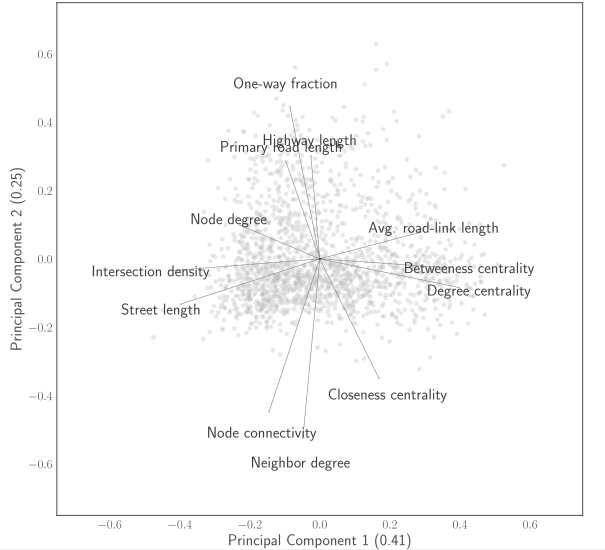
\includegraphics[height=0.75\textwidth]{images/2_revisao/merchan_variables.png}
         \label{fig:merchanVariables}
     \end{subfigure}
     \begin{subfigure}{.49\textwidth}
       \centering
       \caption{Projeção da clusterização sobre a ACP}
       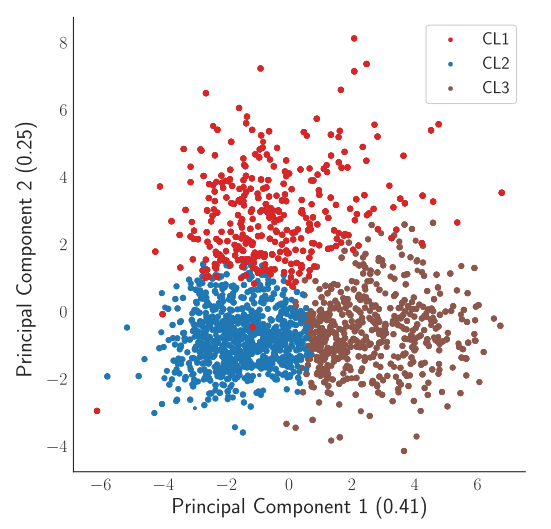
\includegraphics[height=0.75\textwidth]{images/2_revisao/merchan_clusterized.png}
       \label{fig:merchanClusterized}
     \end{subfigure}
     \caption*{\ Fonte: \citeonline{merchan2020quantifying}}
\end{figure}

A distribuição espacial dos três diferentes grupos pode ser observada na Figura \ref{fig:merchanSP}, em que se destaca a presença do grupo $CL3$ em regiões periféricas, e do grupo $CL1$ em regiões centrais.

\begin{figure}[htb]
    \centering
    \caption{Resultado do agrupamento com base nas variáveis explanatórias}
    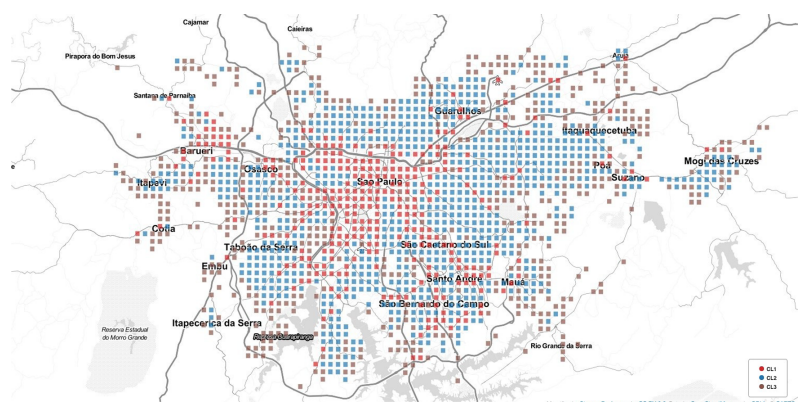
\includegraphics[width=0.9\textwidth]{images/2_revisao/merchan_sp_example.png}
    \caption*{\ Fonte: \citeonline{merchan2020quantifying}}
    \label{fig:merchanSP}
\end{figure}

A partir daí, um modelo de regressão quadrática múltipla é proposto para explicar o fator de circuito a partir das variáveis calculadas, sendo calculada uma regressão para cada grupo $CL1$, $CL2$ e $CL3$.
A determinação dos coeficientes da regressão é realizada através de aprendizagem de máquina, utilizando ferramentas como o \textit{Scikit-learn} (\citeauthoronline{pedregosa2011scikit}, \citeyear{pedregosa2011scikit}).
A partir dos coeficientes, são diferenciadas as variáveis que contribuem para o aumento do fator de circuito (e.g. comprimento de vias, porcentagem de vias de mão única) das variáveis que possuem relação inversa ao fator de circuito, ou seja, que diminuem o valor do fator de circuito quando estas têm seus valores aumentados (e.g. conectividade dos nós).
Por fim, o efeito de cada variável para o valor final do fator de circuito é então discutido, possibilitando a compreensão das considerações finais do trabalho, que podem ser resumidas da seguinte forma:
%
\begin{itemize}
    \item A eficiência de viagens de última milha, neste caso representada pelo fator de circuito, pode ser explicada por uma série de propriedades geométricas e topológicas, algumas das quais podem variar consideravelmente ao longo de uma cidade;
    \item A descrição com base em uma única medida não é suficiente para representar a heterogeneidade da eficiência de viagens de última milha ao longo da cidade, portanto deve-se buscar um conjunto de variáveis que possam descrever diferentes aspectos da malha viária;
    \item A presença de vias de alta capacidade (i.e. rodovias ou vias arteriais) aumenta os valores de fator de circuito no interior das zonas analisadas, que possuem 1 $km^{2}$ de área cada uma.
    Caso fossem analisadas viagens que cruzam a cidade de um extremo ao outro, o resultado seria o oposto: vias de alta capacidade aumentam a eficiência das viagens.
    Ou seja, num contexto de distribuição de última milha, a presença de vias de alta capacidade tende a complicar a eficiência de entregas devido à redução de acessibilidade.
    \item Outros fatores que podem resultar no aumento do fator de circuito são a presença de vias de mão única e a própria topografia local. Por outro lado, malhas viárias de maior índice de conectividade aumentam a acessibilidade e, assim, tendem a apresentar maior eficiência de viagens;
    \item A partir da classificação dos segmentos em três grupos, é possível estabelecer diferentes estratégias de distribuição de entregas, em especial, zonas classificadas como $CL1$ deveriam receber maior atenção ao se projetar sistemas de distribuição de última milha, visto que essas zonas apresentam maiores valores de fator de circuito e maior densidade populacional, implicando em um número maior de entregas sendo realizadas em áreas em que a eficiência de viagens é reduzida.
    \item Um bom entendimento da distribuição espacial do fator de circuito pode contribuir para tomada de decisões em distintas áreas além da logística de distribuição de última milha, tais como o gerenciamento de tráfego e planejamento urbano.
\end{itemize}

%%%%%% Trabalho da Julia: %%%%%%

\citeonline{AMARAL2020102916} também investigaram como a malha viária pode afetar a distribuição de entregas de ultima milha em zonas urbanas, porém desta vez considerando distâncias percorridas, tempo de percurso e topografia da região.
% we propose an approach that allows to identify how the street network within a given urban area may affect last mile distribution in terms of travel distances, travel times and topography
%
São analisadas seis cidades de diferentes continentes e, além disso, é feita uma comparação das velocidades médias de tráfego em diferentes horários do dia.
%
De modo a caracterizar as áreas de estudo, são calculadas variáveis como: densidade de vias ($D_{vias}$), distância média entre quarteirões, densidade de intersecções ($D_{Intersec}$) e porcentagem de vias de mão única ($OW_{ratio}$).
% the following metrics are computed for a preliminary characterization of the study area in terms of its road network: (i) a (iv)

Os resultados obtidos evidenciam a influência que a malha viária exerce sobre as distâncias percorridas em viagens de entregas nas cidades.
% the results we have obtained show that the street network does influence travel distances of delivery trips in the cities.
%
Também pode ser observado que diferentes cidades - as quais possuem diferentes padrões de organização de malha viária - possuem diferentes valores médios de fator de circuito.
% It can also be observed that different cities with different network patterns present different average CFs

Adicionalmente, \citeauthoronline{AMARAL2020102916} explicam que os resultados permitem prever o desempenho da distribuição de entregas nas cidades analisadas. 
% In addition, the results allow a broad comparison between what can be expected from freight deliveries in each city 
%
É citado, como exemplo, que a cidade do Rio de Janeiro possui maior dificuldade de entregas do que as outras cinco cidades estudadas, baseado no maior valor de fator de circuito que essa cidade apresenta.
% For example, it is possible to say that Rio de Janeiro is more challenging for last-mile distribution in terms of traveled distance than the other five cities studied, since it has the highest CFs seen for all distance ranges
%
Nesse sentido, o estudo indica que, durante o planejamento de distribuição de entregas de última milha, uma atenção especial deve ser direcionada para regiões de maior dificuldade de entregas, a fim de se otimizar a eficiência de entregas.
%  at the operational level, special attention should be given to areas deemed as more ‘difficult’ to ensure that the resulting routes are sufficiently robust and less subject to unexpected events
%
Ademais, em relação à evolução da velocidade média dos veículos ao longo do dia, é destacado que em algumas cidades a velocidade média de tráfego tende a variar mais do que em outras e, dessa forma, em determinadas cidades pode ser mais vantajosa a realização de entregas em períodos fora dos horários de pico (e.g. madrugada ou final do dia).  
% Delivery carriers operating in central London, Rio de Janeiro or Bogota would benefit less from switching deliveries to off-hours in terms of vehicle productivity when traveling as travel speed do not increase as much as, for instance, in New York and São Paulo

%%%%%%%%%%%%%%%%%%%%%%%%%%%%%%%%%%%%%%%%%%%%%%%%%%%%%%%
\section{Autocorrelação espacial} \label{sec:autocorrelacaoEsp}

A autocorrelação espacial, como definido por \citeonline{Almeida2012}, busca compreender se existe algum padrão na distribuição espacial dos dados avaliados ou se trata-se de uma distribuição espacialmente aleatória.
A autocorrelação espacial testa a hipótese de que os dados espaciais estão distribuídos aleatoriamente, assim, esta análise faz parte da geoestatística (\citeauthoronline{10.2113/gsecongeo.58.8.1246}, \citeyear{10.2113/gsecongeo.58.8.1246}).

Dentro da geoestatística são estabelecidas diferentes metodologias para a avaliação de autocorrelação espacial dos dados.
A mais tradicional, porém, é a de \citeonline{Moran1948}, que define um coeficiente de autocorrelação espacial conhecido como \textit{I} de Moran.
Sua formulação pode ser observada na Equação \ref{eq:autocor_espacial1}, onde $n$ é o número de regiões utilizadas, $z$ é a variável estudada associada a cada região $i$ e $j$, $W$ é o valor médio das variáveis entre os vizinhos $j$ de $i$ e $S_{0}$ é a média de $z$ globalmente.
%
\begin{equation} \label{eq:autocor_espacial1}
    I = \frac{n}{S_{0}} \cdot \frac{\sum_{i} \sum_{j} W_{ij} Z_{i} Z_{j}}{\sum_{i=1}^{n} Z^2_{i}}
\end{equation}

Sendo assim, a metodologia de \citeauthoronline{Moran1948} busca estabelecer a autocorrelação espacial através do conceito de vizinhança. 
Tal conceito busca compreender, através da variável $z$, se uma região tem algum padrão em relação a seus vizinhos diretos. 
Tal relação é estabelecida a partir da média global ou local a depender da metodologia utilizada.
Na global, categoriza-se cada região como estando acima ou abaixo da média de todos os $z$ observados na área de estudo. 
Já na metodologia local, avalia-se se cada região está acima ou abaixo da média estabelecida entre ela e seus vizinhos diretos.

Após a identificação de cada região em relação à media (global ou local), classifica-se a região de acordo com as seguintes categorias: \textit{Low-Low}, \textit{Low-High}, \textit{High-High}, \textit{High-Low} ou \textit{Indefinido}.
Ao tratar de uma região, por exemplo, que esteja acima da média e seus vizinhos todos abaixo da média, a região é categorizada como \textit{High-Low} e assim por diante.
Se a região não pôde estabelecer algum padrão para com seus vizinhos, ela é classificada como \textit{Indefinida}.
Em termos práticos, \citeauthoronline{Moran1948} permite identificar áreas que possuem padrões de $z$ bem estabelecidos, bem como áreas de baixo padrão espacial (i.e. de disposição geográfica aleatória), que serão classificadas como \textit{Indefinidas}. As representações gráficas dessa classificação das regiões é chamada de Mapa LISA (Mapa de indicadores locais de associação espacial, em tradução livre).

Portanto, a autocorrelação espacial será empregada neste trabalho de modo a investigar a relação entre diferentes zonas, que poderão ser bairros ou cidades, para com os seus vizinhos diretos.

%%%%%%%%%%%%%%%%%%%%%%%%%%%%%%%%%%%%%%%%%%%%%%%%%%%%%%%
\section{Considerações finais sobre a literatura}

Parte dos trabalhos até aqui resultaram em contribuições que evidenciam a interferência das malhas viárias, principalmente com respeito à sua ``circuicidade'', sobre a eficiência das viagens intra urbanas.
Apesar de que algumas outras obras também poderiam ser mencionadas, (e.g. \citeonline{SHEIKHMOHAMMADZADEH2013285}, \citeonline{WANG2020144} e \citeonline{choi2021effect}), a maioria delas trata ou de transporte público urbano ou de viagens de modo automobilístico que não seja relacionado à distribuição de entregas.
%
Além disso, os estudos mencionados na seção \ref{sec:MalhaViariaBiblio} se limitaram a representar a eficiência de entregas de última milha através da medida de fator de circuito, sem de fato entender se essa variável é suficiente para explicar o desempenho dos resultados de roteirizações.

Nesse sentido, não se encontram com facilidade referências que tenham investigado o impacto dessas variáveis sobre a aderência ao sequenciamento programado de entregas. 
Em especial, a literatura deixa espaço para trabalhos que unam a análise espacial de malhas viárias com o desempenho de roteirizações realizadas.
Essa limitação da literatura atual é perfeitamente explicável visto que, se por um lado os dados necessários para a análise espacial são obtidos muitas vezes de banco de dados acessíveis na internet (e.g. \textit{OpenStreetMap}), dados de sequenciamento de entregas são bem mais escassos, visto que estão associados a empresas privadas e que podem conter informações sensíveis tais como o endereço de clientes. 

Em outras palavras, identifica-se a possibilidade de investigação sobre a relação entre os temas de roteirização (\textit{Vehicle Routing Problem}) e disposição espacial de malhas urbanas.
Tal estudo pode contribuir para diferentes áreas de conhecimento, tais como gerenciamento de tráfego, saúde (roteirização de ambulâncias), educação (roteirização de ônibus escolares), entre outros.
Contudo, será dado um foco à distribuição de entregas de última milha, uma vez que esta configura um aspecto menos explorado pela literatura atual.

